% !TEX program = pdflatex
% !TEX encoding = UTF-8 Unicode

\documentclass{beamer}
\usepackage[utf8]{inputenc}
\usepackage[T1]{fontenc}
\usepackage{lmodern}
\usepackage{amsmath,amssymb}
\usepackage{graphicx}
\usepackage{booktabs}
\usepackage{hyperref}
\usepackage{tikz}
\usetikzlibrary{arrows.meta, positioning, shapes.geometric}

\usetheme{Madrid}
\usecolortheme{default}

\definecolor{darkblue}{RGB}{0,51,102}
\definecolor{lightblue}{RGB}{173,216,230}
\setbeamercolor{structure}{fg=darkblue}

%------------------------------------------------------------
\title[BDH Searchless Chess]{BDH-GPU for Searchless Chess}
\subtitle{Proposal Presentation}
\author{Antoni Czapski}
\institute[]{Project: Deep Learning}
\date{March 10, 2026}

%------------------------------------------------------------
\begin{document}

%------------------------------------------------------------
\frame{\titlepage}

%==============================================================================
% SLIDE 1 — Problem
%==============================================================================
\begin{frame}
\frametitle{Problem: Searchless Chess}

\begin{columns}
\column{0.55\textwidth}

\textbf{Input:} Chess board position (FEN)\\
\textbf{Output:} Position score $\in [-1, 1]$\\
\textbf{Task:} Supervised regression

\vspace{1em}
No minimax. No alpha-beta. No MCTS.\\
\alert{Pure neural pattern recognition.}

\vspace{1em}
\textbf{My angle:} Train a novel \alert{post-transformer} architecture (BDH-GPU) and compare against ViT.

\column{0.45\textwidth}
\begin{block}{Prior Art}
\footnotesize
\begin{tabular}{lrc}
\toprule
\textbf{Model} & \textbf{Params} & \textbf{ELO} \\
\midrule
DeepMind '24 & 270M & 2895 \\
ViT-Med$^*$ & 9.5M & 1960 \\
ViT-Small$^*$ & 2.6M & 1817 \\
ResNet-XL$^*$ & 24.7M & 1719 \\
\bottomrule
\end{tabular}

\vspace{0.3em}
{\tiny $^*$Grzyb, 2025 --- open dataset \& models}
\end{block}
\end{columns}

\end{frame}

%==============================================================================
% SLIDE 2 — Why BDH
%==============================================================================
\begin{frame}
\frametitle{Why BDH-GPU?}

\begin{block}{BDH in one sentence}
Recurrent linear-attention model with \alert{Hebbian fast-state updates} and \alert{shared weights across layers}.
\end{block}

\vspace{0.5em}
\textbf{Three reasons it fits chess:}

\begin{enumerate}
    \item \textbf{Relational state} --- piece interactions (pins, forks, batteries) stored as neuron-pair synaptic weights
    \item \textbf{Iterative reasoning} --- same layer applied $K$ times = ``thinking longer'' about hard positions
    \item \textbf{Sparse activations} --- only relevant patterns fire, natural match for chess motifs
\end{enumerate}

\vspace{0.5em}
\begin{center}
\alert{No prior work has applied BDH to chess or any game domain.}
\end{center}

\end{frame}

%==============================================================================
% SLIDE 3 — Dataset
%==============================================================================
\begin{frame}
\frametitle{Dataset}

\begin{columns}
\column{0.5\textwidth}
\textbf{Lichess-Stockfish-Normalized}\\
{\footnotesize \url{huggingface.co/datasets/mateuszgrzyb/lichess-stockfish-normalized}}

\vspace{0.5em}
\begin{tabular}{lr}
\toprule
Positions & 316M \\
Format & Parquet (10 shards) \\
License & CC BY 4.0 \\
I use & $\sim$50--100M subset \\
\bottomrule
\end{tabular}

\vspace{0.5em}
Split: 90\% / 5\% / 5\% (seed \texttt{2001})

\column{0.5\textwidth}
\begin{block}{Encoding}
FEN $\rightarrow$ \texttt{8$\times$8$\times$12} binary tensor\\[0.3em]
\footnotesize 64 squares $\times$ 12 piece channels\\
Always-white perspective
\end{block}

\vspace{0.5em}
\begin{block}{Pipeline}
\footnotesize
HuggingFace download $\rightarrow$ encode $\rightarrow$ split $\rightarrow$ TFRecord streaming
\end{block}

\vspace{0.5em}
\begin{block}{Key}
\footnotesize
Proven dataset --- already produced 1960 ELO models. Direct comparability.
\end{block}
\end{columns}

\end{frame}

%==============================================================================
% SLIDE 4 — Architecture + Metric
%==============================================================================
\begin{frame}
\frametitle{Architecture \& Evaluation}

\begin{columns}
\column{0.55\textwidth}

\begin{center}
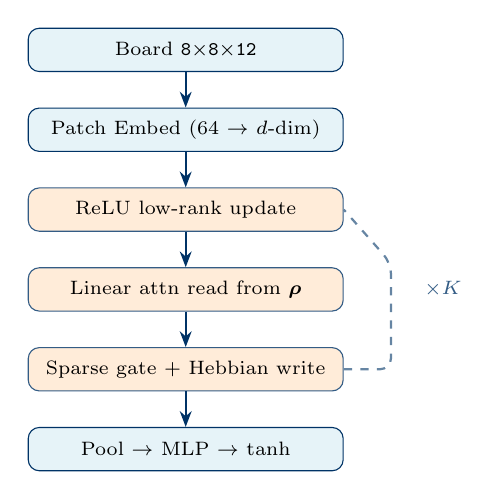
\begin{tikzpicture}[
    node distance=0.45cm,
    box/.style={rectangle, draw=darkblue, fill=lightblue!30, rounded corners,
                minimum height=0.55cm, minimum width=4cm, align=center, font=\scriptsize},
    recbox/.style={rectangle, draw=darkblue!80, fill=orange!15, rounded corners,
                minimum height=0.55cm, minimum width=4cm, align=center, font=\scriptsize},
    arrow/.style={-{Stealth[length=2mm]}, thick, darkblue},
    loopline/.style={thick, darkblue!60, dashed}
]
\node[box] (input) {Board \texttt{8$\times$8$\times$12}};
\node[box, below=of input] (embed) {Patch Embed (64 $\rightarrow$ $d$-dim)};
\node[recbox, below=of embed] (s1) {ReLU low-rank update};
\node[recbox, below=of s1] (s2) {Linear attn read from $\boldsymbol{\rho}$};
\node[recbox, below=of s2] (s3) {Sparse gate + Hebbian write};
\node[box, below=of s3] (head) {Pool $\rightarrow$ MLP $\rightarrow$ $\tanh$};

\draw[arrow] (input)--(embed);
\draw[arrow] (embed)--(s1);
\draw[arrow] (s1)--(s2);
\draw[arrow] (s2)--(s3);
\draw[arrow] (s3)--(head);

\node[right=0.9cm of s2, font=\scriptsize\bfseries, text=darkblue!80] {$\times K$};
\draw[loopline, rounded corners] (s3.east)--++(0.6,0)--++(0,1.35)--(s1.east);
\end{tikzpicture}
\end{center}

\column{0.45\textwidth}
\textbf{Model variants:}
\begin{table}
\centering
\scriptsize
\begin{tabular}{lcc}
\toprule
& \textbf{Params} & $K$ \\
\midrule
BDH-Tiny & 1.6M & 4 \\
BDH-Small & 6.3M & 8 \\
BDH-Medium & 12.6M & 12 \\
\bottomrule
\end{tabular}
\end{table}

\textbf{Baselines:} MLP ($\sim$2M), ViT-Small (2.6M)

\vspace{0.5em}
\textbf{Metrics:}
\begin{itemize}
    \footnotesize
    \item MSE (training loss)
    \item \alert{ELO estimation} via 1200 Lichess puzzles (50\% accuracy threshold)
\end{itemize}
\end{columns}

\end{frame}

%==============================================================================
% SLIDE 5 — Engineering
%==============================================================================
\begin{frame}[fragile]
\frametitle{Engineering \& DevOps}

\begin{columns}
\column{0.5\textwidth}

\begin{block}{\texttt{uv} + Config-driven training}
\scriptsize
\begin{verbatim}
uv sync
uv run python scripts/training/train.py \
  --config configs/train_bdh_small.yaml
\end{verbatim}
\end{block}

\begin{block}{CI/CD (GitHub Actions)}
\footnotesize
\begin{itemize}
    \item \texttt{ruff} --- lint + format
    \item \texttt{pytest} --- 5+ test cases
    \item On every push \& PR
\end{itemize}
\end{block}

\begin{block}{Tests (\texttt{pytest})}
\footnotesize
\begin{itemize}
    \item Data loading \& encoding
    \item BDH forward pass + shapes
    \item Loss sanity + training smoke
\end{itemize}
\end{block}

\column{0.5\textwidth}

\begin{block}{Reproducibility}
\footnotesize
\begin{itemize}
    \item Seeds in YAML $\rightarrow$ \texttt{tf}, \texttt{np}, \texttt{random}
    \item Fixed splits (saved to JSON)
    \item \texttt{uv.lock} pinned deps
    \item \texttt{ModelCheckpoint} best model
\end{itemize}
\end{block}

\begin{block}{W\&B ($\geq$7 experiments)}
\footnotesize
\begin{enumerate}
    \item MLP baseline
    \item ViT-Small baseline
    \item BDH-Tiny
    \item BDH-Small
    \item Depth ablation ($K$=4,8,12)
    \item BDH-Medium
    \item Adaptive depth
\end{enumerate}
\end{block}
\end{columns}

\end{frame}

%==============================================================================
% SLIDE 6 — Timeline & Risks
%==============================================================================
\begin{frame}
\frametitle{Compute, Timeline \& Risks}

\begin{columns}
\column{0.5\textwidth}
\textbf{100h on NVIDIA A100:}
\begin{table}
\centering
\scriptsize
\begin{tabular}{lr}
\toprule
\textbf{Task} & \textbf{Hours} \\
\midrule
Data pipeline + baselines & 9h \\
BDH-Tiny (iteration) & 5h \\
BDH-Small (main) & 20h \\
Depth ablation & 15h \\
BDH-Medium & 40h \\
Eval + buffer & 11h \\
\midrule
\textbf{Total} & \textbf{100h} \\
\bottomrule
\end{tabular}
\end{table}

\footnotesize\textit{BDH-Medium is expendable if behind schedule.}

\column{0.5\textwidth}
\textbf{Key risks:}

\begin{alertblock}{\footnotesize BDH underperforms ViT}
\scriptsize Still valid as architecture comparison. Strong baselines ensure contribution.
\end{alertblock}

\begin{alertblock}{\footnotesize No reference implementation}
\scriptsize Start tiny, unit-test everything, verify gradients early.
\end{alertblock}

\vspace{0.3em}
\textbf{Meeting roadmap:}
\scriptsize
\begin{tabular}{cl}
4 & Repo + CI green \\
5 & EDA + baselines \\
6--7 & BDH training + W\&B \\
8--9 & Ablations + error analysis \\
10--11 & Scale-up + polish \\
12 & Final presentation \\
\end{tabular}
\end{columns}

\end{frame}

%==============================================================================
% SLIDE 7 — Summary
%==============================================================================
\begin{frame}
\frametitle{Summary}

\begin{center}
\large
\begin{tabular}{rl}
\textbf{Problem} & Searchless chess position evaluation \\[0.5em]
\textbf{Dataset} & 316M positions (HuggingFace, CC BY 4.0) \\[0.5em]
\textbf{Architecture} & BDH-GPU --- post-transformer with Hebbian state \\[0.5em]
\textbf{Metric} & MSE + ELO via 1200 puzzle benchmark \\[0.5em]
\textbf{Engineering} & \texttt{uv} + CI + \texttt{ruff} + \texttt{pytest} + W\&B + YAML \\[0.5em]
\textbf{Compute} & 100h on NVIDIA A100 \\
\end{tabular}
\end{center}

\vspace{1em}
\begin{center}
\Large \textbf{Questions?}
\end{center}

\end{frame}

\end{document}
